
% \yj{same push?}
% \begin{table*}[t]
% \centering
% \footnotesize
% \setlength{\tabcolsep}{6pt}
% \renewcommand{\arraystretch}{1.15}
% \caption{Main results on six mathematical reasoning benchmarks.
% This table reports Avg@8 and Pass@8 accuracy for Qwen3-1.7B and Qwen3-4B models. \method~demonstrates stable performance improvements across benchmarks.}
% \resizebox{\textwidth}{!}{
% \begin{tabular}{>{\centering\arraybackslash}m{3.2cm}*{12}{>{\centering\arraybackslash}m{1.25cm}}}
% \toprule
% \multirow{2}{*}{\textbf{Method}}
% & \multicolumn{2}{c}{\textbf{MATH500}}
% & \multicolumn{2}{c}{\textbf{AMC23}}
% & \multicolumn{2}{c}{\textbf{Minerva}}
% & \multicolumn{2}{c}{\textbf{OlympiadBench}}
% & \multicolumn{2}{c}{\textbf{AIME24}}
% & \multicolumn{2}{c}{\textbf{AIME25}} \\
% \cmidrule(lr){2-3}\cmidrule(lr){4-5}\cmidrule(lr){6-7}
% \cmidrule(lr){8-9}\cmidrule(lr){10-11}\cmidrule(lr){12-13}
% & Avg@8 & Pass@8
% & Avg@8 & Pass@8
% & Avg@8 & Pass@8
% & Avg@8 & Pass@8
% & Avg@8 & Pass@8
% & Avg@8 & Pass@8 \\
% \midrule
% \multicolumn{13}{c}{\textbf{Qwen3-1.7B-Base (MATH)}} \\
% \midrule
% FKL            & 63.80 & 84.20 & 38.11 & 70.00 & 28.14 & 44.10 & 27.66 & 48.40 & \underline{10.06} & 20.00 & 3.36 & 16.67 \\
% GRPO            & \textbf{68.83} & 84.60 & \underline{40.62} & 70.00 & 29.46 & \underline{48.16} & 29.89 & 50.81 & 9.17 & 20.00 & 4.58 & 16.67 \\
% OPD            & 67.76 & \underline{84.80} & 39.06 & 70.00 & \underline{29.83} & 47.06 & 30.09 & \textbf{51.56} & 8.33 & 20.00 & \textbf{6.25} & 16.67 \\
% \midrule
% \textbf{\method}
%                 & \underline{68.73} & \textbf{87.60} & \textbf{41.88} & \textbf{75.00} & \textbf{30.15}& \textbf{50.74} & \textbf{30.28} & \underline{51.11} & \textbf{10.42} & \textbf{23.33} & \underline{5.83} & 16.67 \\
% \midrule
% \multicolumn{13}{c}{\textbf{Qwen3-4B-Base (DAPO-Math-14k)}} \\
% \midrule
% FKL            & 74.73 & 92.20 & 48.13 & \underline{85.00} & 34.65 & 55.15 & 37.33 & \underline{62.52} & 12.50 & 30.00 & 12.08 & 23.33 \\
% GRPO            & \textbf{80.47} & 91.00 & \underline{58.44} & 75.00  & \textbf{40.81} & \underline{55.51} & \textbf{43.37} & 60.74 & 14.85 & 30.00 & \underline{12.66} & 26.67 \\
% OPD            & 78.81 & 90.8 & 57.33 & 80.06 & \underline{40.08} & 54.00 & 
% 42.10 & 58.80 & \textbf{18.33} & 26.67 & 12.08 & \underline{30.00} \\
% \midrule
% \textbf{\method}
%                 & \underline{80.20} & \textbf{93.00} & \textbf{60.94} & \textbf{87.50} & 39.71 & \textbf{56.99} & \underline{43.24} & \textbf{63.11} & \underline{17.92} & \textbf{36.67} & \textbf{17.50} & \textbf{33.33} \\
% \bottomrule
% \end{tabular}
% }
% \label{tab:main_results}
% \end{table*}


\begin{table*}[!t]
\centering
\small

\caption{Main results (accuracy \%) on six mathematical reasoning benchmarks. \method~demonstrates consistent improvements across benchmarks and model scales.  Parentheses indicate training data. \textbf{Bold} indicates best performance and \underline{underline} indicates second-best.}
\resizebox{\textwidth}{!}{
\begin{tabular}{ll*{4}{c}*{4}{c}*{4}{c}}
\toprule
\multirow{2}{*}{\textbf{Benchmark}} & \multirow{2}{*}{\textbf{Metric}} 
& \multicolumn{4}{c}{\textbf{Qwen3-0.6B-Base (MATH)}} 
& \multicolumn{4}{c}{\textbf{Qwen3-1.7B-Base (MATH)}} 
& \multicolumn{4}{c}{\textbf{Qwen3-4B-Base (DAPO-Math-14k)}} \\
\cmidrule(lr){3-6} \cmidrule(lr){7-10} \cmidrule(lr){11-14}
 & 
 & \textbf{KD} & \textbf{GRPO} & \textbf{OPD} & \textbf{\method~(ours)}
 & \textbf{KD} & \textbf{GRPO} & \textbf{OPD} & \textbf{\method~(ours)}
 & \textbf{KD} & \textbf{GRPO} & \textbf{OPD} & \textbf{\method~(ours)} \\
\midrule
\multirow{2}{*}{MATH500}
    & Avg@8  
    & 47.80 & \underline{51.83} & 50.09 &
    \cellcolor{blue!10} \textbf{52.02} 
    & 63.80 & \textbf{68.83} & 67.76 & \cellcolor{blue!10}\underline{68.73} 
    & 74.73 & \textbf{80.47} & 78.81 & \cellcolor{blue!10}\underline{80.20} \\
    & Pass@8 
    & 69.60 & \underline{74.40} & 73.20 & 
    \cellcolor{blue!10} \textbf{76.00} 
    & 84.20 & 84.60 & \underline{84.80} & \cellcolor{blue!10}\textbf{87.60} 
    & \underline{92.20} & 91.00 & 90.80 & \cellcolor{blue!10}\textbf{93.00} \\
\midrule
\multirow{2}{*}{AMC23}
    & Avg@8  
    & 23.43 & \underline{25.25} & 24.69 & 
    \cellcolor{blue!10} \textbf{27.81} 
    & 38.11 & \underline{40.62} & 39.06 & \cellcolor{blue!10}\textbf{41.88} 
    & 48.13 & \underline{58.44} & 57.33 & \cellcolor{blue!10}\textbf{60.94} \\
    & Pass@8 
    & 52.50 & \underline{55.00} & \textbf{57.50} & 
    \cellcolor{blue!10} \underline{55.00} 
    & \underline{70.00} & \underline{70.00} & \underline{70.00} & \cellcolor{blue!10}\textbf{75.00} 
    & \underline{85.00} & 75.00 & 80.00 & \cellcolor{blue!10}\textbf{87.50} \\
\midrule
\multirow{2}{*}{Minerva}
    & Avg@8  
    & 18.61 & \underline{20.08} & 19.98 & 
    \cellcolor{blue!10} \textbf{20.82} 
    & 28.14 & 29.46 & \underline{29.83} & \cellcolor{blue!10}\textbf{30.15} 
    & 34.65 & \textbf{40.81} & \underline{40.08} & \cellcolor{blue!10}39.71 \\
    & Pass@8 
    & \underline{36.03} & 35.66 & 34.93 & 
    \cellcolor{blue!10} \textbf{37.13} 
    & 44.10 & \underline{48.16} & 47.06 & \cellcolor{blue!10}\textbf{50.74} 
    & 55.15 & \underline{55.51} & 54.00 & \cellcolor{blue!10}\textbf{56.99} \\
\midrule
\multirow{2}{*}{OlympiadBench}
    & Avg@8  
    & 18.15 & 18.91 & \textbf{20.15} & 
    \cellcolor{blue!10} \underline{19.52} 
    & 27.66 & 29.89 & \underline{30.09} & \cellcolor{blue!10}\textbf{30.28} 
    & 37.33 & \textbf{43.37} & 42.10 & \cellcolor{blue!10}\underline{43.24} \\
    & Pass@8 
    & 36.59 & 34.96 & \underline{37.19} & 
    \cellcolor{blue!10} \textbf{39.56} 
    & 48.40 & 50.81 & \textbf{51.56} & \cellcolor{blue!10}\underline{51.11} 
    & \underline{62.52} & 60.74 & 58.80 & \cellcolor{blue!10}\textbf{63.11} \\
\midrule
\multirow{2}{*}{AIME24}
    & Avg@8  
    & 2.19 & \textbf{4.58} & 2.50 &
    \cellcolor{blue!10} \underline{4.17} 
    & \underline{10.06} & 9.17 & 8.33 & \cellcolor{blue!10}\textbf{10.42} 
    & 12.50 & 14.85 & \textbf{18.33} & \cellcolor{blue!10}\underline{17.92} \\
    & Pass@8 
    & 6.67 & \underline{10.00} & \underline{10.00} & 
    \cellcolor{blue!10} \textbf{13.33}  
    & \underline{20.00} & \underline{20.00} & \underline{20.00} & \cellcolor{blue!10}\textbf{23.33} 
    & \underline{30.00} & \underline{30.00} & 26.67 & \cellcolor{blue!10}\textbf{36.67} \\
\midrule
\multirow{2}{*}{AIME25}
    & Avg@8  
    & \underline{0.83} & \underline{0.83} & \textbf{1.25} & 
    \cellcolor{blue!10}\textbf{1.25} 
    & 3.36 & 4.58 & \textbf{6.25} & \cellcolor{blue!10}\underline{5.83} 
    & 12.08 & \underline{12.66} & 12.08 & \cellcolor{blue!10}\textbf{17.50} \\
    & Pass@8 
    & \underline{6.67} & \textbf{10.00} & \underline{6.67} & 
    \cellcolor{blue!10}\underline{6.67}
    & 16.67 & 16.67 & 16.67 & \cellcolor{blue!10}16.67 
    & 23.33 & 26.67 & \underline{30.00} & \cellcolor{blue!10}\textbf{33.33} \\
\bottomrule
\end{tabular}
}
\label{tab:main_results}
\end{table*}




\section{Experiments}
\label{sec:experiments}
We address the following research questions:
\begin{enumerate}[leftmargin=2.7em, itemsep=0.2mm, topsep=1pt]
  \item[\textcolor{text_green}{\textbf{RQ1:}}] Does \method~improve mathematical reasoning performance compared to existing baselines? (\S\ref{sec:math_main})
  \item[\textcolor{text_green}{\textbf{RQ2:}}] Does \method~improve out-of-domain performance compared to existing baselines? (\S\ref{sec:ood})
  \item[\textcolor{text_green}{\textbf{RQ3:}}] How does \method~affect the transfer of token-level uncertainty from the teacher to the student? (\S\ref{sec:token_level_entropy})
  \item[\textcolor{text_green}{\textbf{RQ4:}}] How does \method~differ from other entropy-promoting methods in transferring teacher uncertainty? (\S\ref{sec:comparison_entropy_driven})
\end{enumerate}
%\vspace{-1mm}
\subsection{Experimental Settings} \label{sec:experimental_settings}
\textbf{Models and Training Datasets.}
We conduct experiments using three Qwen3~\cite{yang2025qwen3} student models of different sizes, Qwen3-0.6B-Base, Qwen3-1.7B-Base, and Qwen3-4B-Base. We use Qwen3-8B as the teacher model, without enabling thinking mode. For the 0.6B and 1.7B student models, training was performed using the MATH~\cite{hendrycks2021measuring} dataset, while for the 4B student model, the more challenging DAPO~\cite{yu2025dapo} dataset is used.

\textbf{Evaluation Benchmarks and Metrics.}
We evaluate our models on MATH500~\cite{hendrycks2021measuring}, AIME24/25~\cite{maa_aime}, AMC23~\cite{maa_amc}, Minerva~\cite{lewkowycz2022solving}, and OlympiadBench~\cite{he2024olympiadbench}, using a rollout temperature of 1.0, top-$p$ sampling with $p = 0.8$, and a maximum response length of 8192 tokens.
We sample 8 responses per question and report the average accuracy (Avg@8) and pass rate (Pass@8).
% We further evaluate the boundary of reasoning capability using the Pass@$k$ metric by sampling $K$ responses per prompt.
% To mitigate variance, we adopt the unbiased estimation method proposed by Chen et al.~\cite{chen2021evaluating}.

\textbf{Baselines.}
We compare our method with several baselines: 
\begin{enumerate}[leftmargin=1em, itemsep=0.2mm, topsep=1pt]
\item  \textbf{Knowledge Distillation}~\cite{hinton2015distilling, kim2016sequence}: KD trains the student model by minimizing forward KL divergence with respect to the teacher's distribution, along with a cross-entropy loss on hard labels from an off-policy dataset generated by the teacher.
\item \textbf{On-Policy Distillation}~\cite{lu2025onpolicydistillation}: The student is trained using on-policy trajectories, following the formulation described in \S\ref{sec:opd_witch_crkl}.
\item \textbf{Group Relative Policy Optimization (GRPO)}~\cite{shao2024deepseekmath}: GRPO optimizes the policy by comparing verifiable rewards across multiple sampled outputs for the same input. 
% Although GRPO is not a distillation method, it is closely related to on-policy distillation in that the student generates its own trajectories. Moreover, GRPO has been shown to outperform supervised approaches; therefore, we include it as a baseline.
\end{enumerate}
\textbf{Implementation.}
For off-policy distillation (KD), we utilize the DistillKit~\cite{distillkit2024} framework. On-policy distillation and GRPO are implemented using the \texttt{verl}~\cite{sheng2024hybridflow} framework. We train with a batch size of $B=128$ and a mini-batch size of $B_{\text{mini}}=32$, resulting in 4
gradient steps per training iteration. Full implementation details are provided in \autoref{app:implementation_details}.

\subsection{Main Results}

\textbf{Performance on Mathematical Reasoning.}\label{sec:math_main}
As shown in ~\autoref{tab:main_results}, \method~demonstrates stable performance improvements across six mathematical reasoning benchmarks, achieving improved or competitive results in terms of Avg@8 and Pass@8. In particular, compared to OPD, \method~improves Avg@8 by $+1.16$ and Pass@8 by $+1.37$ on average across the six benchmarks for the Qwen3-0.6B-Base model, Avg@8 by $+0.99$ and Pass@8 by $+2.39$ for the Qwen3-1.7B-Base model, and $+1.80$ in Avg@8 and $+5.05$ in Pass@8 for the Qwen3-4B-Base model. These improvements highlight the effectiveness of \method, particularly its ability to better transfer the teacher's local uncertainty.


\begin{figure*}[t]
  \centering
  \begin{subfigure}{0.33\textwidth}
    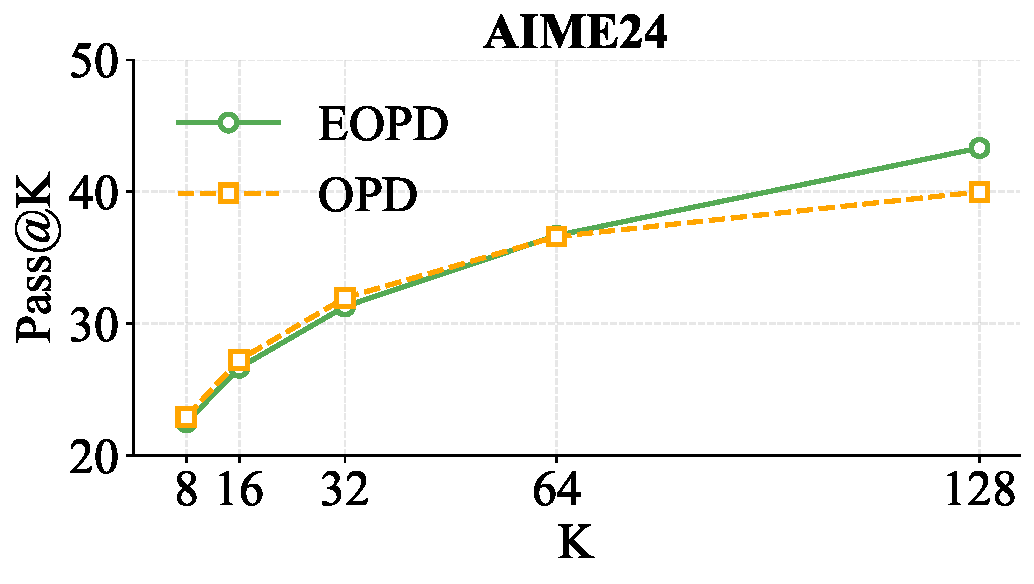
\includegraphics[width=\linewidth]{figure/pass_1.7B_AIME24.pdf}
    %\caption{Qwen3-1.7B-Base}
  \end{subfigure}
  \hfill
  \begin{subfigure}{0.33\textwidth}
    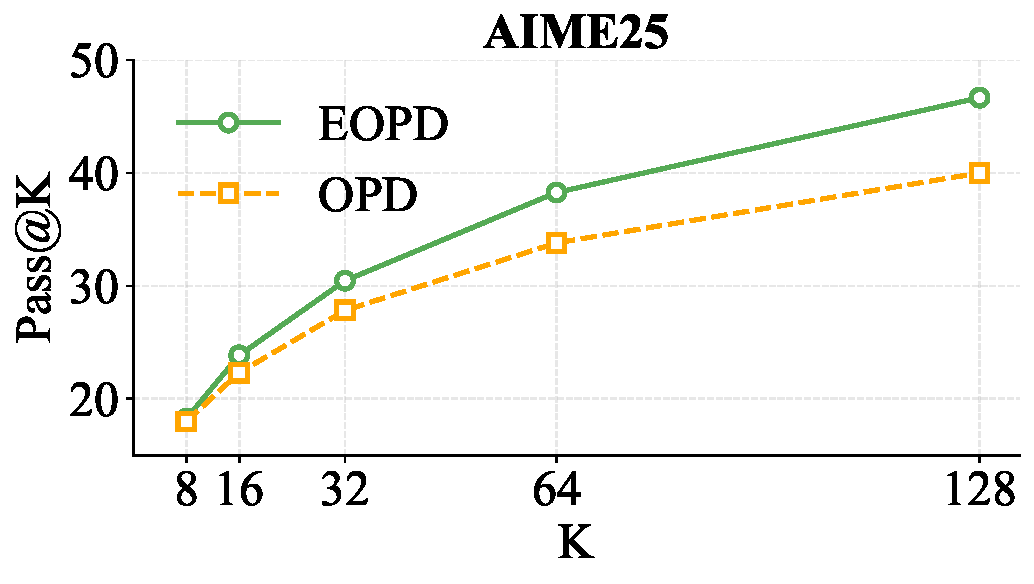
\includegraphics[width=\linewidth]{figure/pass_1.7B_AIME25.pdf}
  \end{subfigure}
  \hfill
  \begin{subfigure}{0.33\textwidth}
    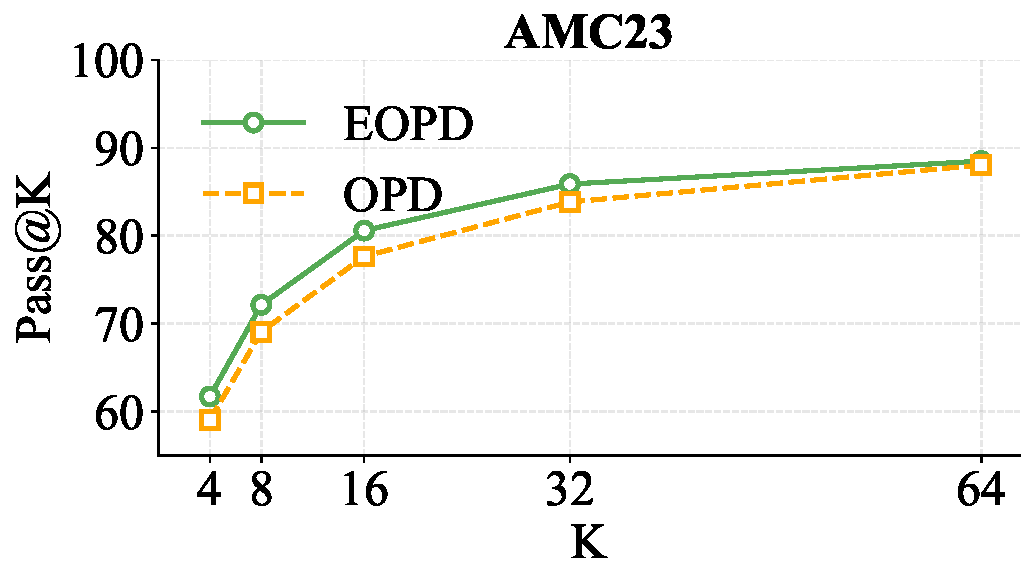
\includegraphics[width=\linewidth]{figure/pass_1.7B_AMC23.pdf}
  \end{subfigure}

  \caption{Pass@$k$ performance comparison between OPD and \method~on the AIME and AMC benchmarks with the Qwen3-1.7B-Base student.
\method~achieves higher Pass@$k$ compared to OPD, with the performance gap becoming more pronounced as $k$ increases.}
  \label{fig:pass_main}
  \vspace{-5pt}
\end{figure*}

\textbf{Pass@$k$ Performance.}\label{sec:pass@k}
Pass@$k$ measures the probability of obtaining at least one correct solution among $k$ sampled rollouts. While Avg@$k$ reflects average reasoning quality, Pass@$k$ more directly captures the model's problem-solving capability by approximating best-case performance under multiple samples.
In \autoref{fig:pass_main}, we report Pass@$k$ for AIME24 and AIME25 with $k$ ranging from 8 to 128, and for AMC23 with $k$ ranging from 4 to 64.
\method~achieves consistently higher Pass@k compared to OPD.
Notably, on harder benchmarks such as AIME, the gap between the two methods widens as $k$ increases.
This suggests that \method~more effectively explores diverse reasoning trajectories, thereby increasing the likelihood of reaching a correct solution. See \autoref{app:pass_others} for more results on Pass@k performance.

% To leverage this capability assessment, we report Pass@$k$ for AIME24 and AIME25 with $k$ ranging from 8 to 128, and for AMC23 with $k$ ranging from 4 to 64. 
% For AIME24 and AIME25, we report Pass@$k$ with $k$ ranging from 8 to 128. For AMC23, we report Pass@$k$ with $k$ ranging from 4 to 64. 
% For efficiency, we sample using the largest value of $k$, then use the unbiased estimation method proposed by \citet{chen2021evaluating} to estimate Pass@$k$ for smaller $k$.
% For challenging benchmarks such as AIME, where single-sample accuracy is low, we report Pass@$k$ for $k = 8$ to $128$ to examine performance under a wide range of sampling budgets. In contrast, for AMC23, where accuracy saturates relatively early due to higher baseline performance, we report results for $k = 4$ to $64$. 

% As shown in \autoref{fig:pass}, \method~achieves overall higher Pass@k compared to OPD. Notably, on harder benchmarks such as AIME, the performance gap between the two methods becomes more pronounced as $k$ increases. This suggests that models trained with \method~more effectively explore diverse reasoning trajectories, therefore increasing the likelihood of reaching a correct solution.





% \begin{table}[ht]
% \centering
% \caption{Out-of-domain benchmark evaluation for Qwen3-1.7B-Base student. We observe that \method~ demonstrates improved performance relative to other baselines. \textbf{Bold} indicates best performance and \underline{underline} indicates second-best.}
% \resizebox{0.45\textwidth}{!}{
% \begin{tabular}{c ccc cc}
% \toprule
% \multirow{2}{*}{Methods}
%  & \multicolumn{2}{c}{\textbf{GPQA-Diamond}}
%  & \multicolumn{1}{c}{\textbf{MMLU-Pro}}
%  & \multicolumn{2}{c}{\textbf{AlpacaEval 2.0}} \\
% \cmidrule(lr){2-3} \cmidrule(lr){4-4} \cmidrule(lr){5-6}
%  & Avg@8 & Pass@8 & Pass@1 & LC-WR & WR \\
% \midrule
% KD     & 27.01\% & 75.20\% & 37.54\% & 19.30\% & 23.63\% \\
% GRPO   & 27.86\% & \underline{77.83\%} & 41.46\% & 16.86\% & 20.55\% \\
% OPD    & \underline{30.08\%} & 77.78\% & \underline{42.26\%} & \underline{22.86\%} & \textbf{29.92\%} \\
% \method& \textbf{31.50\%} & \textbf{81.31\%} & \textbf{43.20\%} & \textbf{23.83\%} & \underline{29.54\%} \\
% \bottomrule
% \end{tabular}
% }
% \label{tab:ood_results}
% \end{table}

\begin{table}[ht]
\centering
% \caption{Out-of-domain benchmark results on Qwen3-1.7B-Base student. \method~demonstrates improved performance relative to other baselines. All values are in \%. WR: win rate; LC-WR: length-controlled win rate. \textbf{Bold} indicates best performance and \underline{underline} indicates second-best.}
\caption{Out-of-domain benchmark results on Qwen3-1.7B-Base, covering general reasoning and instruction following.
Our method achieves higher average accuracy and pass@8 on general reasoning, and is competitive or superior in win rate (\textit{WR}) and length-controlled win rate (\textit{LC-WR}). Best and second-best results are shown in \textbf{bold} and \underline{underline}, respectively.}
\resizebox{0.45\textwidth}{!}{
\begin{tabular}{ll cccc}
\toprule
\textbf{Benchmark} & \textbf{Metric} & \textbf{KD} & \textbf{GRPO} & \textbf{OPD} & \textbf{\method} \\
\midrule
\multirow{2}{*}{GPQA-Diamond} 
 & Avg@8  & 27.01 & 27.86 & \underline{30.08} & \cellcolor{blue!10}\textbf{31.50} \\
 & Pass@8 & 75.20 & \underline{77.83} & 77.78 & \cellcolor{blue!10}\textbf{81.31} \\
\midrule
MMLU-Pro & Pass@1 & 37.54 & 41.46 & \underline{42.26} & \cellcolor{blue!10}\textbf{43.20} \\
\midrule
\multirow{2}{*}{AlpacaEval 2.0} 
 & LC-WR & 19.30 & 16.86 & \underline{22.86} & \cellcolor{blue!10}\textbf{23.83} \\
 & WR    & 23.63 & 20.55 & \textbf{29.92} & \cellcolor{blue!10}\underline{29.54} \\
\bottomrule
\end{tabular}}
\vspace{-3mm}
\label{tab:ood_results}
\end{table}

\subsection{Out-of-domain Evaluation} \label{sec:ood}
\autoref{tab:ood_results} reports performance on out-of-domain benchmarks for the Qwen3-1.7B-Base student: GPQA-Diamond~\cite{rein2024gpqa}, MMLU-Pro~\cite{wang2024mmlu}, and AlpacaEval 2.0~\cite{dubois2024length}, which evaluate general reasoning and instruction-following abilities. Although trained exclusively on math data, OPD and \method~exhibit stable performance increases over KD and GRPO across these benchmarks, indicating that on-policy distillation transfers useful reasoning behaviors beyond the training distribution.

Furthermore, \method~outperforms OPD on all out-of-domain benchmarks except for AlpacaEval 2.0 win rate. This suggests that selectively incorporating teacher guidance on high-uncertainty tokens also provides additional benefits for general reasoning and instruction-following.

% This suggests that on-policy distillation enables effective transfer beyond the training domain.
% In contrast, GRPO relies on verifiable rewards and performs reinforcement learning without teacher guidance, optimizing specifically for the mathematical domain. As a result, GRPO tends to exhibit lower performance on out-of-domain evaluations.



\subsection{Token-Level Entropy Analysis}
\label{sec:token_level_entropy}
To support the hypothesis that \method~more effectively explores diverse reasoning trajectories, we conduct a token-level analysis of uncertainty transfer from the Qwen3-8B teacher to the Qwen3-1.7B-Base student. Following \S\ref{sec:diversity}, we compare students trained with OPD and \method~on the AIME24 and AIME25 benchmarks.

For each generated token, we compute the entropy of the model's predicted distribution conditioned on the preceding context. \autoref{fig:entropy_histogram} aggregates these values into a histogram. In the mid-entropy range (approximately $0.1$–$1.0$), OPD and \method~exhibit similar distributions and remain close to the teacher. The key difference emerges at higher entropy values (entropy $\ge 1.0$): \method~retains substantially more probability mass in this region and stays much closer to the teacher, whereas OPD markedly under-represents it.
% Figure~\ref{fig:entropy_histogram} plots the entropy histogram over token positions.
% Across the mid-entropy regime (roughly $0.1$--$1.0$), OPD and \method~ exhibit broadly similar mass and both remain close to the teacher.
% However, a clear difference emerges in the high-entropy tail: for entropy $\ge 1.0$, \method~preserves substantially more probability mass and stays much closer to the teacher, whereas OPD under-represents this region.

High-entropy tokens correspond to intrinsically ambiguous decision points where the teacher assigns non-negligible probability to multiple plausible continuations. Therefore, preserving a teacher-like distribution at these positions is likely important. We hypothesize that \method’s improved preservation of high-entropy tokens mitigates premature over-confidence and mode collapse, contributing to the downstream performance gains observed in \S\ref{sec:math_main}.
% Since high-entropy tokens correspond to intrinsically ambiguous decision points where the teacher considers multiple plausible continuations. Therefore, maintaining a teacher-like distribution is likely crucial for performance.
% We therefore hypothesize that \method's ability to better preserve this high-entropy regime reduces premature over-confidence and mode collapse, contributing to the observed downstream gains.


% \begin{figure}[t]
%     \centering
%     \includegraphics[width=\linewidth]{figure/dynamics_entropy.pdf}
%     \caption{dynamics: entropy}
%     \label{fig:dynamics_entropy}
% \end{figure}
\begin{figure}[t]
    \centering
    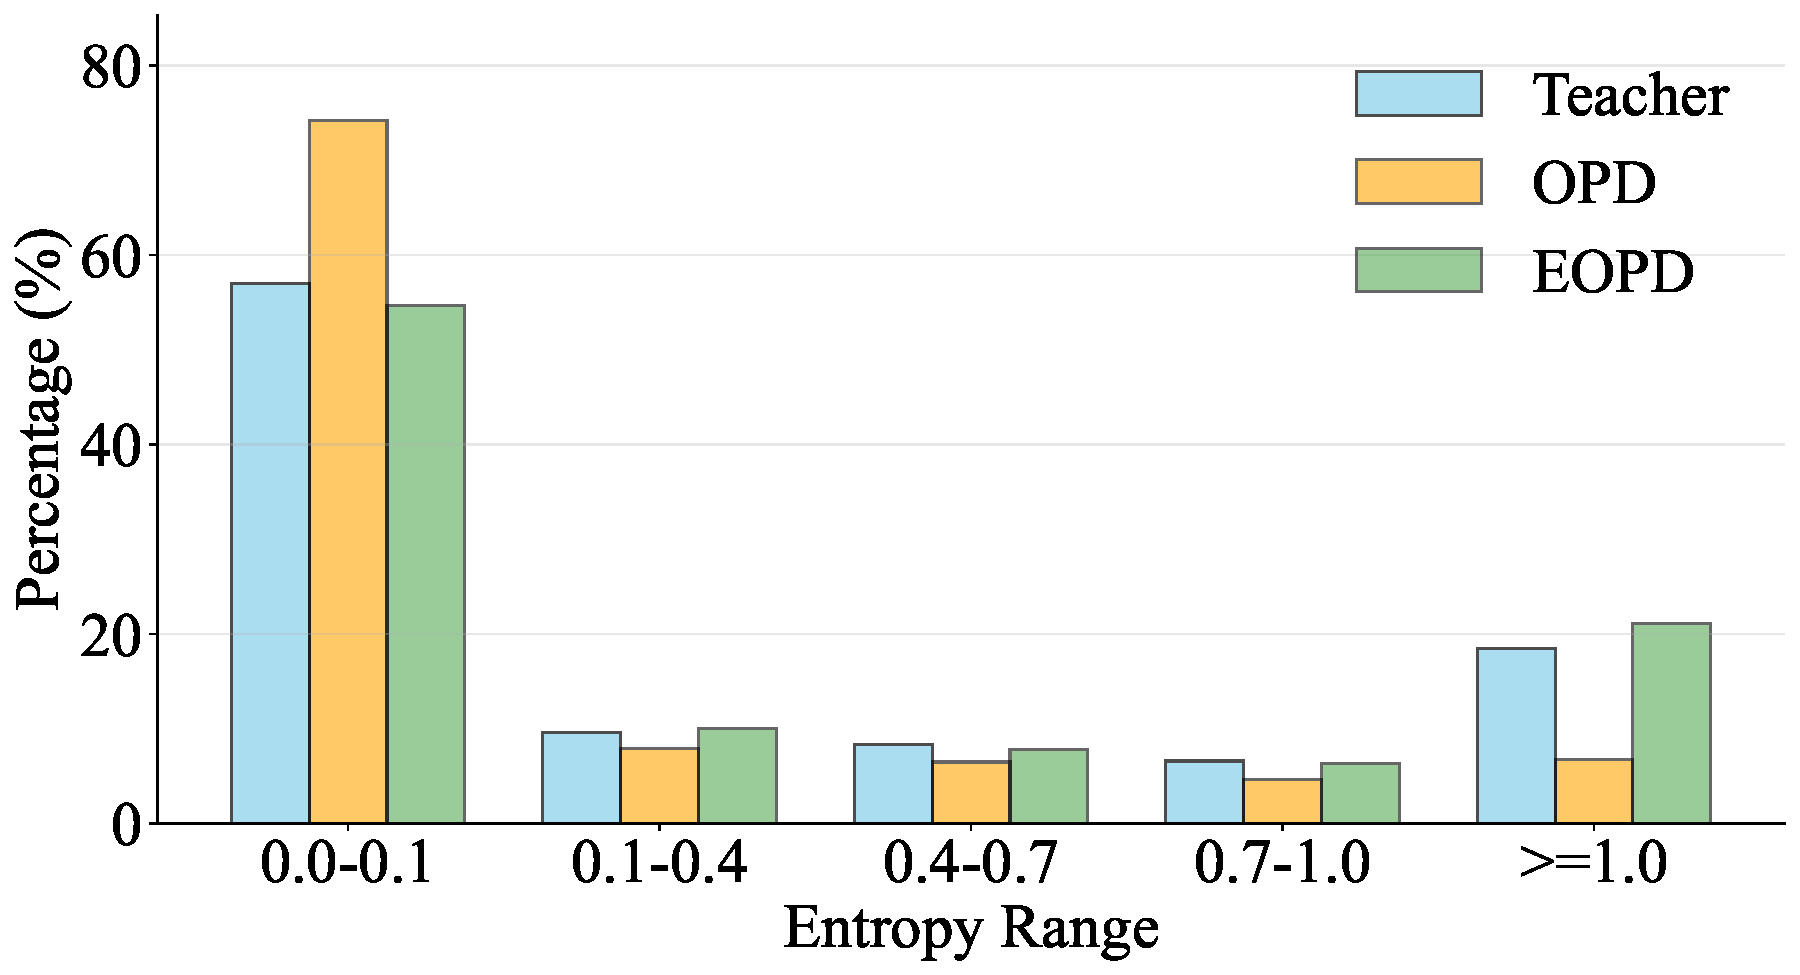
\includegraphics[width=\linewidth]{figure/entropy_distribution_comparison.pdf}
    \caption{Token-level entropy histograms comparing the Qwen3-8B teacher with Qwen3-1.7B-Base trained using OPD and \method~on the AIME 2024 and 2025 benchmarks. While both methods exhibit similar distributions to the teacher in the mid-entropy range, \method~preserves more probability mass in the high-entropy region, staying closer to the teacher than OPD.}
    \label{fig:entropy_histogram}
\end{figure}
\paragraph{}
\begin{figure}[t]
    \centering
    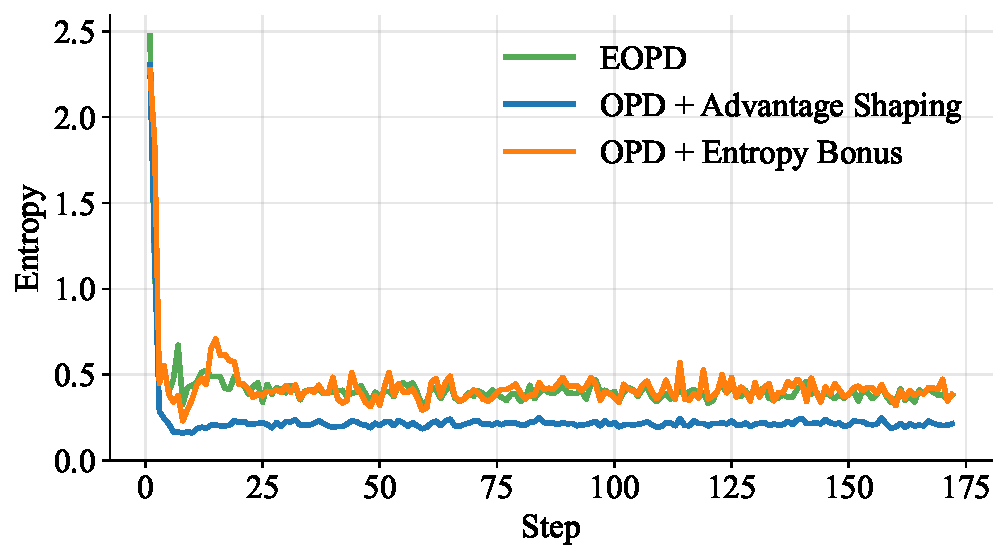
\includegraphics[width=\linewidth]{figure/entropy_curve_analysis.pdf}
    \caption{Average policy entropy during training for the Qwen3-1.7B-Base student trained with OPD + Entropy Bonus, OPD + Advantage Shaping, and \method. Advantage Shaping converges to a lower entropy regime, while Entropy Bonus maintains entropy levels comparable to \method.}
    \label{fig:analysis_entropy}
\end{figure}
\begin{figure}[t]
    \centering
    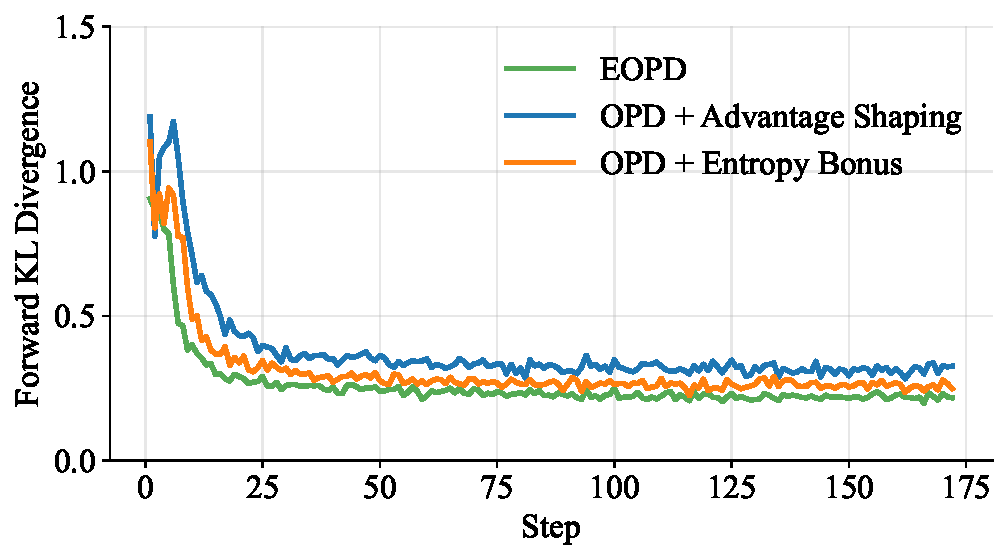
\includegraphics[width=\linewidth]{figure/fkl_curve_compare.pdf}
    \caption{Average forward KL divergence measured during training at token positions where the teacher distribution exhibits high entropy (entropy $\ge 0.8$) for the Qwen3-1.7B-Base student. Compared to OPD + Entropy Bonus and OPD + Advantage Shaping, \method~maintains lower forward KL values throughout training, indicating closer alignment with the teacher distribution in regions of high uncertainty.}
    \label{fig:analysis_fkl}
    %\vspace{-0.3cm}
\end{figure}
\vspace{-3mm}
\subsection{Comparison with Entropy-Driven Baselines}
\label{sec:comparison_entropy_driven}
% \begin{table}[ht]
% \centering
% \caption{Comparison with entropy-driven exploration baselines on MATH500 and AMC23. \method~achieves higher Avg@8 and Pass@8 compared to OPD + Entropy Bonus and OPD + Advantage Shaping.
% }
% \resizebox{0.45\textwidth}{!}{
% \begin{tabular}{c cccc}
% \toprule
% \multirow{2}{*}{Method} 
%  & \multicolumn{2}{c}{\textbf{MATH500}} 
%  & \multicolumn{2}{c}{\textbf{AMC23}} \\
% \cmidrule(lr){2-3} \cmidrule(lr){4-5}
%  & Avg@8 & Pass@8 & Avg@8 & Pass@8 \\
% \midrule
% Entropy Bonus & 66.87\% & 86.00\% & 39.69\% & 75.00\% \\
% Advantage Shaping & 67.90\% & 85.20\% & 36.56\% & 75.00\% \\
% \method & 68.73 \% & 87.60\% & 41.88\% & 75.00\% \\
% \bottomrule
% \end{tabular}
% }
% \label{tab:ablation_entropy_baseline}
% \end{table}

\begin{table}[ht]
\centering
\caption{Comparison with entropy-driven exploration baselines for the Qwen3-1.7B-Base student. \method~achieves higher Avg@8 and Pass@8 compared to OPD + Entropy Bonus and OPD + Advantage Shaping. \textbf{Bold} indicates best performance and \underline{underline} indicates second-best.
}
\resizebox{0.38\textwidth}{!}{
\begin{tabular}{c c c c c}
\toprule
\multirow{2}{*}{\textbf{Benchmark}} & \multirow{2}{*}{\textbf{Metric}}
& \textbf{Entropy} & \textbf{Advantage} & \multirow{2}{*}{ \textbf{\method}}\\
&  & \textbf{Bonus} & \textbf{Shaping} & \\
\midrule
\multirow{2}{*}{MATH500}
& Avg@8  & 66.87 & \underline{67.90} & \cellcolor{blue!10}\textbf{68.73} \\
& Pass@8 & \underline{86.00} & 85.20 & \cellcolor{blue!10}\textbf{87.60} \\
\addlinespace
\midrule
\multirow{2}{*}{AMC23}
& Avg@8  & \underline{39.69} & 36.56 & \cellcolor{blue!10}\textbf{41.88} \\
& Pass@8 & \textbf{75.00} & \textbf{75.00} & \cellcolor{blue!10}\textbf{75.00} \\
\addlinespace
\midrule
\multirow{2}{*}{AIME24}
& Avg@8 & \underline{9.58} & 8.75 & \cellcolor{blue!10}\textbf{10.42} \\
& Pass@8 & \underline{20.00} & \textbf{23.33} & \cellcolor{blue!10}\textbf{23.33} \\
\addlinespace
\midrule
\multirow{2}{*}{AIME25}
& Avg@8  & \underline{4.58} & \textbf{5.83} & \cellcolor{blue!10}\textbf{5.83} \\
& Pass@8 & \underline{16.67} & \textbf{20.00} & \cellcolor{blue!10}\underline{16.67} \\
\bottomrule
\end{tabular}}
%\vspace{-0.4cm}
\label{tab:ablation_entropy_baseline}
\end{table}

We compare our method with entropy-based approaches commonly used to encourage exploration in reinforcement learning. 
Specifically, we evaluate the Qwen3-1.7B-Base student using two strategies: an entropy bonus~\citep{schulman2017proximal}, which explicitly regularizes the policy toward higher entropy, and advantage shaping~\citep{cheng2025reasoning}, which augments the advantage with an entropy-dependent term to bias updates toward high-uncertainty actions.
% Specifically, we consider adding to the Qwen3-1.7B-Base student an entropy bonus~\citep{schulman2017proximal}, which explicitly regularizes the policy toward higher entropy, or advantage shaping~\citep{cheng2025reasoning}, which augments the advantage with an entropy-dependent term to bias updates toward high-uncertainty actions.
% Specifically, we consider adding an entropy bonus~\citep{schulman2017proximal} (OPD + Entropy Bonus) and advantage shaping~\citep{cheng2025reasoning} (OPD + Advantage Shaping) to the Qwen3-1.7B-Base student. 
Detailed implementation details are provided in \autoref{app:implementation_details}.

As shown in \autoref{tab:ablation_entropy_baseline}, \method~outperforms both baselines across several benchmarks.
% MATH500, AMC23, AIME24, and AIME25. 
To explain these gains, we analyze entropy dynamics (\autoref{fig:analysis_entropy}) and forward KL at high-entropy positions (\autoref{fig:analysis_fkl}).
OPD + Advantage Shaping exhibits substantially lower training entropy than other methods, indicating limited diversity and explaining its poor performance. However, \method~and OPD + Entropy Bonus maintain similar entropy levels, so entropy alone does not explain \method's advantage. Looking at the forward KL at positions where the teacher's entropy exceeds $\tau=0.8$, \method~achieves consistently lower values than OPD + Entropy Bonus, indicating better alignment with the teacher in uncertain regions. Overall, these results show that preserving entropy alone is insufficient for the student to match the teacher’s diversity, especially in high-entropy regions.


% As shown in \autoref{tab:ablation_entropy_baseline}, \method~outperforms both baselines on the MATH500, AMC23, AIME24 and AIME25 benchmarks under the Avg@8 and Pass@8 metrics. To understand why, we analyze entropy dynamics during training (\autoref{fig:analysis_entropy}). Models trained with OPD + Advantage Shaping exhibit lower training entropy than \method, while OPD + Entropy Bonus results in training entropy levels comparable to \method.
% To assess alignment with the teacher distribution in regions of uncertainty, we report the forward KL divergence on high-entropy token positions in~\autoref{fig:analysis_fkl}. For student-generated sequences, we compute the average forward KL loss at token positions where the teacher distribution has entropy greater than a threshold $\tau=0.8$. This metric evaluates how well the student matches the teacher’s probability distribution in uncertain regions. The results show that \method~consistently achieves lower forward KL values than both baseline methods, indicating better alignment with the teacher distribution where uncertainty is highest.
% % ~\autoref{fig:analysis_fkl} shows the forward KL loss measured at token positions where the teacher distribution has higher entropy than $\tau$ during training. For sequences generated by the student, the average forward KL value is computed at token positions with high entropy under the teacher distribution. This metric evaluates how well the student approximates the teacher’s probability distribution in regions where the teacher exhibits uncertainty. The results show that \method consistently achieves lower forward KL values than all compared methods.
% Overall, these results indicate that simply preserving entropy does not guarantee that the student exhibits diversity similar to the teacher's, particularly in the teacher’s high-entropy regions.
% % These results suggest that approaches which preserve or increase entropy without an explicit target distribution do not guarantee diversity aligned with the teacher distribution.

\subsection{Comparison with GKD} \label{sec:gkd}
We compare \method~with GKD~\cite{agarwal2024policy}, which optimizes a divergence objective over a mixture of off-policy data and on-policy rollouts controlled by a coefficient $\lambda$. Following GKD, we use forward KL for reasoning experiments.
Specifically, the off-policy data is generated by the teacher model (Qwen3-8B), while the on-policy data is sampled from the student (Qwen3-1.7B-Base) during training. We evaluate $\lambda \in \{0.5, 0.8, 1.0\}$.
We observe that the fully on-policy setting ($\lambda = 1.0$) achieves the best performance among different $\lambda$ values, consistent with GKD’s observation that on-policy rollouts are particularly important for reasoning tasks. As shown in~\autoref{tab:gkd}, \method~consistently outperforms the tuned GKD baseline across all benchmarks.
\begin{table}[ht]
\centering
\caption{Comparison with GKD baselines for the Qwen3-1.7B-Base student. We evaluate GKD with different $\lambda$ values following the original setup. \method~consistently outperforms all GKD variants across reasoning benchmarks. \textbf{Bold} indicates best performance and \underline{underline} indicates second-best.}
\resizebox{0.48\textwidth}{!}{
\begin{tabular}{c c c c c c}
\toprule
\multirow{2}{*}{\textbf{Benchmark}} & \multirow{2}{*}{\textbf{Metric}}
& \textbf{GKD} & \textbf{GKD} & \textbf{GKD} & \multirow{2}{*}{\textbf{\method}} \\
& & ($\lambda=0.5$) & ($\lambda=0.8$) & ($\lambda=1.0$) & \\
\midrule
\multirow{2}{*}{MATH500}
& Avg@8  & 64.53 & 65.28 & \underline{67.20} & \cellcolor{blue!10}\textbf{68.73} \\
& Pass@8 & 84.40 & 84.20 & \underline{85.00} & \cellcolor{blue!10}\textbf{87.60} \\
\addlinespace
\midrule
\multirow{2}{*}{AMC23}
& Avg@8  & 35.62 & 37.50 & \underline{38.44} & \cellcolor{blue!10}\textbf{41.88} \\
& Pass@8 & 67.50 & \underline{70.00} & 67.50 & \cellcolor{blue!10}\textbf{75.00} \\
\addlinespace
\midrule
\multirow{2}{*}{AIME24}
& Avg@8 & 5.83 & 6.67 & \underline{9.17} & \cellcolor{blue!10}\textbf{10.42} \\
& Pass@8 & 10.00 & \underline{13.33} & \textbf{23.33} & \cellcolor{blue!10}\textbf{23.33} \\
\addlinespace
\midrule
\multirow{2}{*}{AIME25}
& Avg@8  & 4.58 & 3.75 & \underline{5.00} & \cellcolor{blue!10}\textbf{5.83} \\
& Pass@8 & 10.00 & 10.00 & \underline{13.33} & \cellcolor{blue!10}\textbf{16.67} \\
\bottomrule
\end{tabular}}
\label{tab:gkd}
\end{table}

\subsection{Effect of KL Objective}\label{sec:kl_objective}
To analyze the effect of different KL objectives, we compare \method~with OPD and OPD-FKL using the Qwen3-1.7B-Base student. Here, OPD optimizes the policy using the reverse KL-based reward discussed throughout the paper, while OPD-FKL optimizes the policy using only forward KL under the same on-policy setup.
As shown in \autoref{tab:kl_objective}, reverse KL-based OPD generally outperforms OPD-FKL across most benchmarks, while \method~outperforms both. These results suggest that reverse KL is effective for capturing the dominant modes of the teacher distribution, while selectively applying forward KL in regions with high teacher uncertainty is important for further improving performance.

\begin{table}[ht]
\centering
\caption{
Comparison of different KL objectives for the Qwen3-1.7B-Base student. \method~outperforms both OPD and OPD-FKL across most benchmarks, while OPD generally outperforms OPD-FKL. \textbf{Bold} indicates the best performance and \underline{underline} indicates second-best.
}
\resizebox{0.40\textwidth}{!}{
\begin{tabular}{c c c c c}
\toprule
\textbf{Benchmark} & \textbf{Metric} & \textbf{OPD-FKL} & \textbf{OPD} & \textbf{\method} \\
\midrule
\multirow{2}{*}{MATH500}
& Avg@8  & 67.20 & \underline{67.76} & \cellcolor{blue!10}\textbf{68.73} \\
& Pass@8 & \underline{85.00} & 84.80 & \cellcolor{blue!10}\textbf{87.60} \\
\addlinespace
\midrule
\multirow{2}{*}{AMC23}
& Avg@8  & 38.44 & \underline{39.06} & \cellcolor{blue!10}\textbf{41.88} \\
& Pass@8 & 67.50 & \underline{70.00} & \cellcolor{blue!10}\textbf{75.00} \\
\addlinespace
\midrule
\multirow{2}{*}{AIME24}
& Avg@8  & \underline{9.17} & 8.33 & \cellcolor{blue!10}\textbf{10.42} \\
& Pass@8 & \textbf{23.33} & \underline{20.00} & \cellcolor{blue!10}\textbf{23.33} \\
\addlinespace
\midrule
\multirow{2}{*}{AIME25}
& Avg@8  & 5.00 & \textbf{6.25} & \cellcolor{blue!10}\underline{5.83} \\
& Pass@8 & \underline{13.33} & \textbf{16.67} & \cellcolor{blue!10}\textbf{16.67} \\
\bottomrule
\end{tabular}
}
\label{tab:kl_objective}
\end{table}


\subsection{Impact of Forward KL Placement}\label{sec:fkl_placement}
To study the impact of token selection for application of forward KL, we compare \method~ against two alternative forward KL augmentation strategies for the Qwen3-1.7B-Base student: full forward KL, applied at all token positions, and random forward KL, applied to a randomly selected 20\% of positions\footnote{This choice is motivated by experiments with \method~at $\tau = 0.8$. As shown in \autoref{fig:high_entropy_ratio}, forward KL is applied to approximately 15–20\% of tokens on average.}.
% To analyze how the choice of token positions for applying forward KL affects performance, we compare \method~with two alternative forward KL augmentation strategies for Qwen3-1.7B-Base student. The comparison includes full forward KL, which applies forward KL at all token positions, and random forward KL, which applies forward KL to a randomly selected 20\% of token positions. 
As shown in~\autoref{tab:fkl_placement}, \method~shows competitive performance compared to full and random forward KL. Notably, random forward KL underperforms the other two approaches across most benchmarks, suggesting that the placement of forward KL on appropriate positions, like \method~is important.

\begin{table}[ht]
\centering
\caption{
Comparison with different forward KL placement strategies for the Qwen3-1.7B-Base student. \method~shows competitive performance against full and random forward KL, while random forward KL underperforms the other two approaches. %across benchmarks. 
\textbf{Bold} indicates the best performance and \underline{underline} indicates second-best.
}
\resizebox{0.38\textwidth}{!}{
\begin{tabular}{c c c c c}
\toprule
\textbf{Benchmark} & \textbf{Metric} & \textbf{Full} & \textbf{Random} & \textbf{\method} \\
\midrule
\multirow{2}{*}{MATH500}
& Avg@8  & \underline{67.58} & 67.33 & \cellcolor{blue!10}\textbf{68.73} \\
& Pass@8 & \underline{86.20} & 84.80 & \cellcolor{blue!10}\textbf{87.60} \\
\addlinespace
\midrule
\multirow{2}{*}{AMC23}
& Avg@8  & \underline{39.39} & 36.88 & \cellcolor{blue!10}\textbf{41.88} \\
& Pass@8 & \textbf{75.00} & \underline{67.50} & \cellcolor{blue!10}\textbf{75.00} \\
\addlinespace
\midrule
\multirow{2}{*}{AIME24}
& Avg@8  & \underline{8.75} & 7.92 & \cellcolor{blue!10}\textbf{10.42} \\
& Pass@8 & \textbf{23.33} & \underline{20.00} & \cellcolor{blue!10}\textbf{23.33} \\
\addlinespace
\midrule
\multirow{2}{*}{AIME25}
& Avg@8  & 5.00 & \underline{5.42}  & \cellcolor{blue!10}\textbf{5.83} \\
& Pass@8 & \textbf{20.00} & 13.33 & \cellcolor{blue!10}\underline{16.67} \\
\bottomrule
\end{tabular}
}
%\vspace{-0.4cm}
\label{tab:fkl_placement}
\end{table}

